%%%%%%%%%%%%%%%%%%%%%%%%%%%%%%%%%%%%%%%%%%
\chapter{Introduction} \label{sec:introduction}
%%%%%%%%%%%%%%%%%%%%%%%%%%%%%%%%%%%%%%%%%%
To realize the dream of controlled nuclear fusion, the two large challenges of the engineering of a working reactor must be faced: material of the plasma-facing ``first wall'' and breeding tritium for sustained thermonuclear burns. In this thesis, I hope to make an impact, however small, on the engineering of the latter. 

The first generation of thermonuclear fusion reactors will require reservoirs of tritium for their fuel cycle. Because tritium only exists in minute amounts in nature, the fusion reactor will generate, or ``breed'' from the transmutation of lithium into tritium. A design was proposed by Abdou et al\cite{Abdou1974d} in 1975 wherein the plasma would be surrounded by a so-called blanket of nonmobile, solid lithium. The lithium would be combined with refractory materials to maintain the solid phase at elevated temperatures. In the team since this proposal, the most extensively studied designs see the lithiated ceramic existing in a packed bed of spherical pebbles.

To date, the leading candidates for lithiated ceramic are \lit and \lis. Pebble beds of these materials have been chosen by many participants of the International Thermonuclear Experimental Reactor (ITER) for tritium generation studies.\cite{Lulewicz2002, Mandal2012a, Tsuchiya1998, Cho2012} The advantages of the pebble bed design include ease of uniformly assembling the solid into complex geometries, ease of tritium extraction from the porous bed via an interstitial purge of helium, and with the small size of pebbles being more resilient to thermal stresses than a solid brick of lithiated ceramic.\cite{Casadio2004} Nothing comes without a price, naturally, and there are many issues with pebble bed tritium breeders that must be understood and overcome.

In typical solid breeder modules, coolant fluid runs through the containing structure surrounding the pebble bed. A low-pressure, low-speed purge gas is pumped through the pebble bed to extract the tritium generated and transport it out of the blanket for processing. As nuclear energy is deposited into the poorly-conductive ceramic breeder material, the temperature climbs well above the containing structure. Heat is removed from the pebble bed predominately through inter-particle conduction (with a small contribution from convection of the purge gas) and contact conductance of many pebbles pressed against the containing surface. 

The thermophysical and thermomechanical properties of pebble beds have been studied extensively [cite many of the experimental papers]. From experimental measurements, and the assumption that a pebble bed can be treated as a continuous media, researchers have developed phenomonological formulas relating properties of pebble bed to other, measurable, macroscopic properties [cite many of the modeling papers]. For instance, an effective thermal conductivity can be given for the packed bed given a certain gas and stress on the bed. These effective material properties are useful for the design and qualification of tritium breeding modules. But it must be understood that the material properties of a pebble bed are a function of their history and will evolve in time as the morphological features of the pebble bed likewise evolve in time. Therefore there is a need to predict the morphological changes to the pebble bed and the subsequent impact on the bed's thermophysical properties so that solid breeder designers may have reliable temperature control of the pebble bed over the duration of the use of the breeder in the reactor. 

In the rest of this chapter we will present in more detail the background of solid breeder research and the path we will take to solve some of the design issues of temperature control in solid breeders. We begin in \cref{sec:intro-blanket-description} by setting the foundation of the research with a discussion of the major design requirements and features of a fusion reactor blanket so that it may guide the choices and constraints of research efforts. In \cref{sec:intro-bed-integrity}, we will go into more of the physics and engineering behind the need for- and approaches for maintaining- temperature control in a solid breeder. Finally in \cref{sec:intro-scope-of-work}, the scope of this work will be outlined.




\section{Description of solid breeder blankets}\label{sec:intro-blanket-description}

Before describing the solid breeder blanket and the design requirements, it is worth reviewing the major features of a fusion reaction and potential reactor. The current, worldwide choice for fusion reaction is deuterium-tritium (D-T). The choice is based on D-T having a high reaction probability at the lowest ion temperature, high energy yield, fuel availability, and reaction products (how harmless are the daughter products). The D-T cycle is

\begin{align}
	\mathrm{D} +~\mathrm{T}&\xrightarrow{}~^4\mathrm{He}+\mathrm{n}+17.58~\text{MeV} \label{eq:dt-reaction}
\end{align}

While Deuterium ($D$, or $^2$H), is a stable isotope and is naturally occuring in an average abundance of 0.015 mole percent in water on Earth. Tritium ($T$, or $^3$H), conversely, is radioactive with a half life of only about 12.32 years; naturally decaying as $\beta^-$ emitter (no $\gamma$ rays),

\begin{align}\label{eq:t-decay}
	\mathrm{T} \xrightarrow{}~^3\mathrm{He} + \beta^-
\end{align}
%~~~~~~~~~~~~~~~~~~~~~~~~~~~~~~~~~~~~~~~~~~~~~~~~



%~~~~~~~~~~~~~~~~~~~~~~~~~~~~~~~~~~~~~~~~~~~~~~~~
\subsection{Tritium breeding}

Owing to its short half life, any naturally occurring tritium would decay at such a rapid pace it can never accumulate. Because of this, it will need to be generated artificially (breeded) if it is to be used as a fuel in a fusion reactor. Fusion reactor designs receiving the most attention from the international community include a tritium breeding blanket as an integral component for maintaining self-sufficiency of the reaction. It is achieved with lithium. When natural lithium interacts with a neutron, its two most common isotopes have the following reaction

\begin{align}
	\mathrm{n}_\text{fast} + ~^7\mathrm{Li} &\xrightarrow ~\mathrm{n}+\alpha + \mathrm{T} -2.47~\text{MeV}\label{eq:Li7T}\\
	\mathrm{n}_\text{thermal} + ~^6\mathrm{Li} &\xrightarrow ~ \alpha + \mathrm{T} +4.78~\text{MeV} \label{eq:Li6T}
\end{align}

where we haved used the common short-hand of $\alpha$ in place of the helium nucleus. The cross-sections of the lithium reactions are given in Fig.~\ref{fig:li-xsects}

\begin{figure}
	\centering
	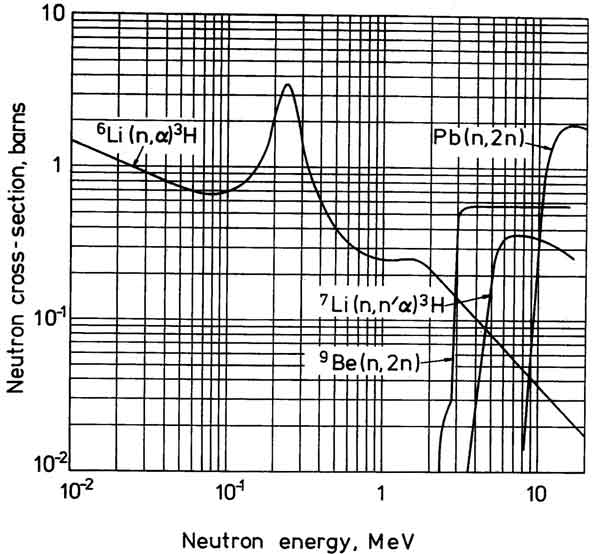
\includegraphics[width=0.8\textwidth]{chapters/figures/breeding_xsecs} 
	\caption{Cross-sections of various blanket materials. Note the threshold for the $^7$Li and neutron multiplying reactions.}
	\label{fig:li-xsects}
\end{figure}

Serendipitously, the D-T reaction itself produces a high energy neutron (see Eq.~\ref{eq:dt-reaction}). If we assume that $D$ is essentially limitless (on the scale of human consumption) and have access to abundant supplies of lithium, then if we complete the fuel cycle of neutron-lithium-tritium, we essentially have an inexhaustible energy source.

One classification of the efficacy of a breeding blanket is through the `tritium breeding ratio' of the fusion powerplant, defined as 

\begin{equation}
	\text{TBR} = \cfrac{\dot{N}^+}{\dot{N}^-}
\end{equation}

where $\dot{N}^+$ is the number of tritium atoms generated per unit time and $\dot{N}^-$ are the number of tritium atoms consumed per unit time.

For a DT cycle, $\dot{N}^- = $~number of fusion reactions in a plasma per unit time (each fusion reaction produces a single neutron). Therefore, for a DT cycle, we have a simplified definition that the tritium breeding ratio is the number of tritium atoms produced in the blanket per fusion neutron. In order to realize fusion as a commercial energy source, it is utterly crucial that the TBR of the plant design be greater than 1.

Clearly it is essential to engineer a device that surrounds the fusion reaction, captures the ejected neutron to breed tritium, and allows recovery of that tritium to attain self-sufficiency. Additionally, the blanket must also be capable of converting energy deposited from neutrons, $\gamma$s, and surface radiation from the plasma and then recovering the energy at high tempreatures for efficient power production in the fusion power plant.

Blanket designs have evolved significantly since their introducetion in the 1970s. Some features of current breeder designs will be discussed next.


% \chapter{Nuclear Design of the Blanket}
% \label{blanketDesign}
% The blanket contains:
% \begin{enumerate}
% \item Tritium breeding material (lithium in some form)
% \item Attenuating materials
% \item Neutron multipliers (in some designs)
% \item Coolant
% \item Structural material
% \item Reflector
% \item Insulators (in some designs)
% \end{enumerate}




%~~~~~~~~~~~~~~~~~~~~~~~~~~~~~~~~~~~~~~~~~~~~~~~~



%~~~~~~~~~~~~~~~~~~~~~~~~~~~~~~~~~~~~~~~~~~~~~~~~
\subsection{Solid breeder design}
Reference current styles of design. edge-on, etc.

% From TOFE-2014
The solid breeder in many current designs for ITER feature sub-module units of packed beds1. From the point of view of pebble bed thermomechanics, this has the advantage of producing units individually that can be tested and qualified to desired packing states (and therefore thermomechanics) during the design phase.

We aim to provide designers of packed beds with tools to understand how packing states may evolve from time-dependent phenomena (e.g. sintering, creep, pebble cracking, etc.). These phenomena may, for instance: decrease the effective thermal conductivity which will raise bed temperatures beyond initial predictions, produce isolated pebbles which will sinter and potentially decrease tritium release rates, or even the form gaps between pebble beds and containing structures leading to divergence from initial packing properties. 
%~~~~~~~~~~~~~~~~~~~~~~~~~~~~~~~~~~~~~~~~~~~~~~~~



%~~~~~~~~~~~~~~~~~~~~~~~~~~~~~~~~~~~~~~~~~~~~~~~~
\subsection{Material candidates and related phenomena}
Lithium can exist in the breeding blanket as either a liquid or a solid. We will limit the scope of our discussion entirely to the solid form. To date, most parties researching solid breeder devices are focusing on lithium orthosilicate (Li$_4$SiO$_4$) or lithium metatitanite (Li$_2$TiO$_3$) as candidate ceramics, though other candidate ceramics do still exist.

Solid breeders are always separately cooled by either water or helium flowing through coolant channels. 

Pure lithium is chemically active meaning safety is an issue. As an example, here are two reactions with oxygen along with their heats of formation
\begin{align*}
	2\mathrm{Li} + \frac{1}{2}\mathrm{O} &\rightarrow \mathrm{Li}_2\mathrm{O} - 142.75~\text{kCal/mol}\\
	2\mathrm{Li} + \mathrm{O} &\rightarrow \mathrm{Li}_2\mathrm{O}_2 - 151.9~\text{kCal/mol}
\end{align*}
note: a negative heat of formation means an exothermic reaction. Lithium will exothermically react with water (or air, concrete, or any moisture-containing materials) with high amounts of energy released. Of primary concern in lithium fires is the peak flame temperature. This will determine, to a large extent, whether many radioactive species become air-borne by vaporization. The flame temperature depends on many variables. Some investigations found it to be  about 2500 K which would cause some materials to melt but not vaporize.


% Neutron multipliers are needed to increase the breeding ratio, particularly in lithium compounds ({e.g.} Li$_4$SiO$_4$). Moreover they increase energy multiplication. Materials to act as neutron multipliers would be those that have large neutron multiplication cross sections (over large energy ranges). They react with (n,2n), (n,3n), or even (n, fission), however the fission reaction is obviously not desirable in a pure fusion reactor. Furthermore it is desirable that they have low neutron absorption and that they would have a favorable impact on energy multiplication. 

% The two most prominently analyzed neutron multipliers for a fusion reactor are beryllium and lead. Beryllium has a very high nuclide density while also being very light, with a high melting temperature, and high thermal conductivity. However it undergoes a 2-$\alpha$ reaction that causes trapped helium to swell the material. There is also a rarely occurring reaction with beryllium that generates tritium; it is frequent enough to cause a concern with contamination.

\section{Pebble Bed Integrity, Thermophysics, and the Role of Modeling}\label{sec:intro-bed-integrity}

The pebble bed will experience a constrained thermal expansion as the hot ceramic pebbles press against the relatively cooler container. The restricted thermal expansion of the pebble bed causes an external pressure on the pebble bed. The external pressure may lead to a number of phenomena that disrupt the initial packing -- and by extension the initial predictions of thermal and mechanical properties -- of the pebble bed. For one, in experiments of even well-packed ensembles of pebbles, the beds show an apparent plastic strain of rearranged packing that increases with maximum historical stress on the bed.[cite Chunbo and Reimanns experimental papers] Without careful engineering and packing of the virgin pebble beds, plastic strain in the pebble bed will directly lead to the formation of gaps between the pebble bed and containing structure. Depending on the configuration of the solid breeder design, the gap could cause a tremendous loss of heat transport from the pebble bed to the coolant. Furthermore, any gaps formed in the blanket could lead to more neutron leakage and decreased tritium breeding ratios and detriment to the blanket's shielding function.

Additionally, assuming that the plastic strain is removed from the pebble bed, the thermally-induced pressure on the pebble bed will be balanced by the individual pebbles pressing into each other at small points of contact. The small area over which the contact forces are applied leads to stresses which may crush individual pebbles in the ensemble. With the potential accumulation of many cracked/crushed individual pebbles, the overall packing structure is again altered. Depending on the extent of crushing, the response of the pebble bed may be as benevolent as a negligible decrease in effective thermal conductivity or malevolent as a loss of physical contact and heat transport from the pebble bed to the coolant. 

Finally there are long-term effects expected in the materials experiencing prolonged exposure to cycling irradiation, heat, and stress. Thermal ratcheting, swelling, sintering, or thermally-induced creep can lead to evolutions in thermophysical properties even in the absence of cracked pebbles. As the thermophysical properties evolve, global or local bed temperatures change and ultimately the tritium release characteristics of the bed deviate from any prediction one may have had from the initial packing of the ceramic pebble bed. 

In our group we are most focused on maintaining tritium breeding characteristics of the pebble bed at desirable levels and thus maintaing temperatures in the breeding region. Alleviating any of the issues that may plague the ceramic breeder all boil down to requiring temperature control via an understanding and of the morphological changes of the ceramic packed beds and their interaction with the interstitial purge gas and structural container. [say how temperature control is possible with better models]In this work we introduce enhancements and new elements to build upon the understanding from ceramic breeder models of past research efforts. 







% Control of the manufacturing processes of the ceramic pebbles permits manufactureres to custom vary characteristics, such as the pebble's:
% \begin{itemize}
% \item tritium retention and release properties.
% \item Lithium density
% \item Opened- and closed-porosity
% \item Nominal diameter
% \item and, indirectly, crush strength. 
% \end{itemize}
% However the characteristics of the pebble are often coupled. For instance, for the sake of tritium management the open porosity of the pebble is often increased. But this comes at the expense of a decreased crush strength of the pebble. Because of the relatively weak crush strength distributions among batches of pebbles as well as the value of stresses predicted in the pebble bed, it is inevitable that during operation in the fusion environment individual pebbles will `fail' in the ensemble. Designers of lithium ceramic tritium breeding blankets must mitigate pebble failure but also anticipate the breadth and magnitude of effects that some unavoidable failure will have on macroscopic properties.



% [EDIT: THIS PARAGRAPH IS NOT NECESSARY? I DON'T NEED TO MAKE THE CASE FOR USING DEM. I JUST NEED TO EXPLAIN THE MODEL]The volume of a pebble in a tritium breeder is on the scale of 10$^{-9}$~m$^3$ while the typical container volume can be on the order of 10$^{-2}$~m$^3$\cite{Cho2008}.  Thus a single breeder volume will house upwards of $N = 10^7$ pebbles. Statistically then, the behavior of any single pebble seems insignificant and instead the entire ensemble of pebbles may be treated as a continuous media. Continuum theory for the is the basis of finite element method models that have been able to predict thermomechanical behavior with reasonable accuracy\cite{DiMaio20081287,Zaccari20081282,Gan:2009vn}. However, after the pebble beds are placed into the fusion environment they will be required to operate for long duty times without maintenance. Thus, as time progresses the accumulation of individual failed pebbles will eventually have consequences for the macroscopic thermomechanics.  and no continuum theory exists to account for this. Instead, we turn to the discrete element method to provide a solutino.

\section{Scope of the work}\label{sec:intro-scope-of-work}
[Here we need an objective (or objectives) first. Perhaps you mention the objective in the middle of the section. It should be clearly written in the beginning of the section-- The objective of this research is to create modeling tools to be able to simulate the pebble bed morphology evolution, and to address consequent heat transfer and temperature, and to provide ----. 

scope of work- 1. to develop a transient DEM code for simulating pebbled bed morphology evolution, 2. to develop DEM coupled CFD code for heat transfer and temperature analysis, 3. to assess thermal mixing using LBM, 4. to apply the developed modeling tools for blanket pebble bed design thermal evaluations, 5. further implication---.]




To develop a complete numerical model for a pebble bed requires completing many interacting sub-models. To demonstrate, we give here the path of a possible analysis scheme of these models. To begin, one must have knowledge of the interaction of the pebble bed with the containing structure as they exist in a fusion environment. The interactions are generally analyzed via the finite element method to find internal stresses and temperature fields of the entirety of the pebble bed and surrounding container. After the internal fields are mapped into the bed, one would use the discrete element method (DEM) to interpret the macroscopic stress fields into the inter-particle forces. With the inter-particle forces and total absorbed thermal energy calculated, a prediction of the initiation and evolution of morphological changes (i.e. crushed pebbles, sintering, creep, etc.) to each computational volume. Following this, DEM would calculate new effective properties as a result of the morphological changes to the pebble bed region. Finally, the updated bed properties would feed back into the FEM formulation to update calculations in the macroscopic stress fields. A suite of integrated numerical tools that follows this example algorithm is the goal of the Fusion Science and Technology Center at UCLA, but we are far from that at this time. The work of this dissertation is focused entirely on the development of pebble-scale simulations that are predominately in the realm of the discrete element method.

We aim to provide designers of packed beds with tools to understand how packing states may evolve from time-dependent phenomena (e.g. sintering, creep, pebble cracking, etc.). These phenomena may, for instance: decrease the effective thermal conductivity which will raise bed temperatures beyond initial predictions, produce isolated pebbles which will sinter and potentially decrease tritium release rates, or even form gaps between pebble beds and containing structures leading to divergence from properties of the initial packing of the bed.

Modeling research on ceramic pebble beds should have as its main objective a thorough understanding of the evolution of pebble bed morphology and the impact on thermo-physical properties; allowing for temperature control of breeder pebble beds over the entire lifetime of the blanket. To accomplish that goal, this current study is aimed at developing a methodology for coupling established discrete element models of individual pebbles in the ensemble with thermo-fluid simulations of the interstitial helium purge gas. Specifically, we will address the impact of helium on the thermal transport in a bed experiencing evolving morphology due to cracked pebbles.

Specifically, much of the work in this dissertation concerns the evolution of thermo-physical properties of a pebble bed in the presence of crushed individual pebbles. When a pebble in an ensemble is crushed or cracked it loses contact with its neighboring pebbles and subsequently breaks any thermal or mechanical transport that the pebble was providing -- ultimately this is manifest in measurable changes to thermo-physical properties. We attempt to quantify the evolving thermo-physical changes with increasingly sophisticated DEM models of ceramic pebble beds.


%DEM
\subsection*{DEM}
In the first study of \cref{sec:dem-studies}, we analyze the effective thermal conductivity of a pebble bed assuming different fractions of pebbles in the ensemble are completely crushed. The focus of this study is to determine the extent of change in aggregate ensemble properties due to individual pebble crushing, relate the changes in effective conductivity to quantifiable pebble-scale properties (e.g. contact force, coordination number, etc.), as well as help designers anticipate acceptable limits of pebble loss from a thermal management point of view. For the DEM tools used in this study, the only mode of heat transfer is conduction between the solid particles. 



%CFD-DEM
\subsection*{CFD-DEM}
In a fusion breeder, the helium purge gas winding through the interstitial gaps of the pebbles has a substantial contribution to overall heat transfer.\cite{Reimann:2002mi,Abou-Sena2005} The model of \cref{sec:dem-studies} is improved to include the flowing interstitial gas. In \cref{sec:cfd-dem-studies}, we continue to employ our DEM tools to provide particle-scale information such as contact force, but couple the pebbles to a volume-averaged computational fluid dynamics (CFD) code. The coupled CFD-DEM model is again used to simulate the heat transfer in packed beds of ceramic spheres that experience pebble crushing -- but now investigate the impact of a flowing interstitial helium purge gas when pebbles are crushed.



%APPLICATION -- ORIENTATION OF CONTAINER
\subsection*{Applied CFD-DEM}
In the study of \cref{sec:applied-studies}, we apply our coupled CFD-DEM computational tools to the analysis of ITER-relevant solid breeder geometries. In this study we consider the combined effects of pebble crushing, packing restructuring due to both gravity and the unbalanced force network in the pebble bed, and convection from helium purge gas on temperature profiles in solid breeders for different breeding configurations. In typical solid breeder modules, coolant fluid runs through the containing structure surrounding the pebble bed. Heat is removed from the pebble bed predominately through inter-particle conduction and contact conductance of many pebbles pressed against the containing surface. As such, heat transfer out of the pebble bed relies on maintaining good pebble-pebble and pebble-wall contact. However, physical contact is interrupted to different degrees when a pebble bed responds to various amounts of individual crushed pebbles. Furthermore, the restructuring of the pebble bed after a pebble crushing event is, in part, dependent on gravity forces acting upon each pebble in the ensemble. We investigate two representative pebble bed configurations where heat is removed from the bed via inter-particle conduction, convection of purge gas, and contact between the pebble bed and its container. In the first, the coolant containing structural walls (heat transfer walls) are oriented parallel to the gravity vector. In the second configuration, the heat transfer walls are perpendicular to the direction of gravity. To simulate a crushed pebble, we replace the pebble with many smaller, non-cohesive elements while maintaining mass-conservation between the original solid pebble and crushed fragments. The fragments are then free to resettle into interstitial gaps and the rest of the bed resettles as determined by forces from gravity, contact of neighboring particles, and even the small influence of the moving purge gas. The thermo-fluid interaction with the helium purge gas will be included with volume-averaged Navier-Stokes and energy equations. The representative solid breeder volumes will be compared with respect to their temperature peaks and profiles and how those temperatures vary as a function of the percentage of crushed pebbles in the ensemble. The results can be used to optimize solid breeder pebble bed designs through the choice of breeding zone orientation relative to the gravity vector.


%LBM
\subsection*{LBM}
The models used to account for helium purge gas in the studies of \cref{sec:cfd-dem-studies,sec:applied-studies} assume effective drag or heat transfer coefficients for pebbles in a computational volume and then include the pebble influence through effective source/sink terms in the momentum and energy equations. The volume-averaged approach allows for simpler meshing of the fluid volume while still retaining much of the physical realism of the system. Complete models of the conjugate heat transfer of both the fluid moving through the tortuous interstitial gaps pebble beds pressing each other with small contact areas are intractable with current computational hardware and finite-element modeling techniques. To overcome deficiencies in computational power, in \cref{sec:modeling-lbm}, we apply the lattice-Boltzmann algorithm to our pebble bed with helium. The lattice-Boltzmann method (LBM) is a non-traditional fluid simulation technique that allows us to resolve pebble-scale interactions with bed-scale conjugate heat transfer with flowing gas on realistic simulation time scales. The LBM approach is applied to the same pebble beds analyzed in \cref{sec:cfd-dem-studies} to provide comparison between the two modeling techniques. Furthermore the LBM model, accounting for the complex helium purge gas pathways, provides more insight to the influence of helium on the heat transfer in the heat transfer of packed beds.


%Background studies
% \subsection*{Other kinds of studies and shit}
% \cref{sec:studies-experiments}
% \cref{sec:studies-numerics}








